\documentclass[
  bibliography=totoc,     % Literatur im Inhaltsverzeichnis
  captions=tableheading,  % Tabellenüberschriften
  titlepage=firstiscover, % Titelseite ist Deckblatt
]{scrartcl}

% Paket float verbessern
\usepackage{scrhack}

% Warnung, falls nochmal kompiliert werden muss
\usepackage[aux]{rerunfilecheck}

% unverzichtbare Mathe-Befehle
\usepackage{amsmath}
% viele Mathe-Symbole
\usepackage{amssymb}
% Erweiterungen für amsmath
\usepackage{mathtools}

% Fonteinstellungen
\usepackage{fontspec}
% Latin Modern Fonts werden automatisch geladen
% Alternativ:
%\setromanfont{Libertinus Serif}
%\setsansfont{Libertinus Sans}
%\setmonofont{Libertinus Mono}
\recalctypearea % Wenn man andere Schriftarten gesetzt hat,
% sollte man das Seiten-Layout neu berechnen lassen

% deutsche Spracheinstellungen
\usepackage{polyglossia}
\setmainlanguage{german}


\usepackage[
  math-style=ISO,    % ┐
  bold-style=ISO,    % │
  sans-style=italic, % │ ISO-Standard folgen
  nabla=upright,     % │
  partial=upright,   % ┘
  warnings-off={           % ┐
    mathtools-colon,       % │ unnötige Warnungen ausschalten
    mathtools-overbracket, % │
  },                       % ┘
]{unicode-math}

% traditionelle Fonts für Mathematik
\setmathfont{Latin Modern Math}
% Alternativ:
%\setmathfont{Libertinus Math}

\setmathfont{XITS Math}[range={scr, bfscr}]
\setmathfont{XITS Math}[range={cal, bfcal}, StylisticSet=1]

% Zahlen und Einheiten
\usepackage[
  locale=DE,                   % deutsche Einstellungen
  separate-uncertainty=true,   % immer Fehler mit \pm
  per-mode=symbol-or-fraction, % / in inline math, fraction in display math
]{siunitx}

% chemische Formeln
\usepackage[
  version=4,
  math-greek=default, % ┐ mit unicode-math zusammenarbeiten
  text-greek=default, % ┘
]{mhchem}

% richtige Anführungszeichen
\usepackage[autostyle]{csquotes}

% schöne Brüche im Text
\usepackage{xfrac}

% Standardplatzierung für Floats einstellen
\usepackage{float}
\floatplacement{figure}{htbp}
\floatplacement{table}{htbp}

% Floats innerhalb einer Section halten
\usepackage[
  section, % Floats innerhalb der Section halten
  below,   % unterhalb der Section aber auf der selben Seite ist ok
]{placeins}

% Seite drehen für breite Tabellen: landscape Umgebung
\usepackage{pdflscape}

% Captions schöner machen.
\usepackage[
  labelfont=bf,        % Tabelle x: Abbildung y: ist jetzt fett
  font=small,          % Schrift etwas kleiner als Dokument
  width=0.9\textwidth, % maximale Breite einer Caption schmaler
]{caption}
% subfigure, subtable, subref
\usepackage{subcaption}

% Grafiken können eingebunden werden
\usepackage{graphicx}
% größere Variation von Dateinamen möglich
\usepackage{grffile}

% schöne Tabellen
\usepackage{booktabs}

% Verbesserungen am Schriftbild
\usepackage{microtype}

% Literaturverzeichnis
\usepackage[
  backend=biber,
]{biblatex}
% Quellendatenbank
\addbibresource{lit.bib}
\addbibresource{programme.bib}

% Hyperlinks im Dokument
\usepackage[
  unicode,        % Unicode in PDF-Attributen erlauben
  pdfusetitle,    % Titel, Autoren und Datum als PDF-Attribute
  pdfcreator={},  % ┐ PDF-Attribute säubern
  pdfproducer={}, % ┘
]{hyperref}
% erweiterte Bookmarks im PDF
\usepackage{bookmark}

% Trennung von Wörtern mit Strichen
\usepackage[shortcuts]{extdash}

\setlength{\parindent}{0em}

\newcommand{\HRule}{\rule{\linewidth}{0.5mm}}
\newcommand{\pii}{\symup{\pi}}

\author{%
  Anneke Reinold%
  \texorpdfstring{%
    \\%
    \href{mailto:anneke.reinold@udo.edu}{anneke.reinold@udo.edu}
  }{}%
  \texorpdfstring{\and}{, }%
  Paul-Simon Blomenkamp%
  \texorpdfstring{%
    \\%
    \href{mailto:paul-simon.blomenkamp@udo.edu}{paul-simon.blomenkamp@udo.edu}
  }{}%
}
\publishers{TU Dortmund – Fakultät Physik}


\begin{document}

\begin{titlepage}
  \begin{flushleft}
 Durchführung: 25.11.2019\\
 1. Abgabe: XX.XX.2019\\
  \end{flushleft}


\HRule\\[1,0cm]

 \begin{center}


\textsc{\LARGE Praktikumsprotokoll V46}\\[1.5cm]
\textsc{\huge Faraday-Effekt} \\[5,5cm]

Anneke Reinold\footnotemark[1], \\
Paul-Simon Blomenkamp\footnotemark[2] \\[1,0cm]



 \end{center}
\HRule

 \vfill
 \footnotetext[1]{\href{mailto:anneke.reinold@tu-dortmund.de}{anneke.reinold@tu-dortmund.de}}
 \footnotetext[2]{\href{mailto:paul-simon.blomenkamp@tu-dortmund.de}{paul-simon.blomenkamp@tu-dortmund.de}}
\end{titlepage}
\section{Einleitung}
Das Ziel dieses Versuchs ist die Bestimmung der effektiven Massen von Kristallelektronen in GaAs durch ausnutzen des Faraday-Effekts. 

\section{Theorie}
\subsection{Von Bändern und Massen}%<-jk......darf ich nicht vergessen zu  ändern
Die physikalische Beschreibung von Elektronen in einem Kristall lässt sich am besten durch die Betrachtung der unteren Bandkante des Leitungsbandes annähern. Es lässt sich dann die Elektronenenergie $\epsilon(\vec{k})$, wobei $\vec{k}$ der Wellenzahlvektor ist, in einer Taylorreihe zu:
\begin{equation}
\epsilon(\vec{k})=\epsilon\left(0\right)+\frac{1}{2}\sum_{i=1}^3\left(\frac{\partial\epsilon^2}{\partial k_i^2}\right)_{k=0}k_i^2+...\,,
\end{equation}
entwickeln.
Vergleicht man dies mit einem harmonischen Oszillator mit
\begin{equation}
  \epsilon=\frac{\hbar k^2}{2m}\,,
\end{equation}
so stellt man fest, dass die Größe:
\begin{equation}
m_i^*:=\frac{\hbar^2}{\left(\frac{\partial\epsilon^2}{\partial k_i^2}\right)_{k=0}}\,,
\end{equation}
die Dimension einer Masse hat. Sie wird auch als effektive Masse des Kristallelektrons bezeichnet.
Für hinreichend hohe Symmentrien des Kristalls sind die einzelnen $m_i^*$ alle gleich groß und das Elektron lässt sich wie ein freies Teilchen mit Masse $m_i^*$ behandeln.
\subsection{Zirkulare Doppelbrechung}
Optische Doppelbrechung bezeichnet die Rotation der Polarisationsebene von linear polarisiertem Licht beim Durchqueren eines Mediums. Physikalisch lässt sich dieses Phänomen nachvollziehen, indem man linear polarisiertes Licht in zwei entgegengesetzt zirkular polarisierte Komponenten zerlegt
\begin{equation}
E(z)=\frac{1}{2}(E_\text{L}(z)+E_\text{R}(z))\,.
\end{equation}
In einem doppeltbrechenden Kristall ist es nun so, dass die Phasengeschwindigkeiten für rechts- und linkszirkular polarisiertes Licht unterschiedlich ist, was zur Polarisationsdrehung um den Winkel $\Theta$ führt. Für eine Welle, welche bei $z=0$ eintritt und in $x$-Richtung polarisiert ist
\begin{equation}
  E(0)=E_0\vec{x_0}\,,
\end{equation}
lässt sich mit
\begin{equation}
  \psi:=\frac{1}{2}\left(k_\text{R})+k_\text{L}\right)
\end{equation}
und
\begin{equation}
\Theta:=\frac{1}{2}\left(k_\text{R})-k_\text{L}\right)
\end{equation}
zeigen, dass sie sich nach einer Länge L durch
\begin{equation}
E(L)=E_0 \exp{\text{i}\psi}\left(\cos(\Theta)\vec{x_0}+\sin(\Theta)\vec{y_0}\right)\,,
\end{equation}
beschreiben lässt.\\
Die Ursache des doppeltbrechenden Verhaltens einiger Kristalle liegt in induzierten Dipolen im Kristall, welche durch das Feld der Strahlung erzeugt werden. Diese verursachen eine makroskopische Polarisierung $\vec{P}$ des Kristalls
\begin{equation}
\vec{P}=\epsilon_0\chi\vec{E}\,,
\end{equation}
wobei $\epsilon_0$ die Influenzkonstante und $\chi$ die dielektrische Suszeptibilität ist.

\section{Durchführung}
\subsection{Versuchsaufbau}
Der genutzte Versuchsaufbau ist in Abb.\ref{Aufbau} dargestellt. Die Lichtquelle des Aufbaus ist eine Halogen-Lampe, welche ein Spektrum hat das größtenteils im Infrarot bereich liegt. Das emittierte Licht wird durch eine Linse gebündelt und durch einen Lichtzerhacker in Pulse eingeteilt.
Die Lineapolarisierung des Lichts erfolgt durch ein Glan-Thompson-Prisma, dessen Winkel zum Strahl durch ein Goniometer variiert werden kann. Die Photonen treffen danach auf die scheibenförmige Probe, welche in einem Elektromagneten mit Feldrichtung parallel zur Photonenrichtung platziert ist. Hinter der Probe befindet sich eine Halterung für austauschbare Interferenzfilter. Zur Untersuchung der Rotation der Polarisationsebene wird die Strahlung mit einem zweiten Glan-Thompson-Prisma in zwei senkrecht zueinander polarisierte Teile  zerlegt und die Teilstrahle werden erneut durch Linsen gebündelt und die Lichtintensität wird mitel Photowiderständen gemessen. Die hohe Rauschspannung welche an den Photowiderständen auftritt wird durch die Wechsellichtmethode, welche durch den Lichtzerhacker und einen auf die Frequenz des Zerhackers eingestellten Selektivverstärker gegeben ist, verhindert. Die am Photowiderstand wird an Kondensatoren ausgegekopplet, wobei die Zeitkonstante von einem der Kondensatoren variabel ist. Die Signale beider Photowiderstände werden aufeinen Differenzverstärker gegeben und von dort in den Selektivverstärker. Das Signal des Selektivverstärkers wird an einem Oszilloskop angezeigt.
\begin{figure}[H]
  \centering
  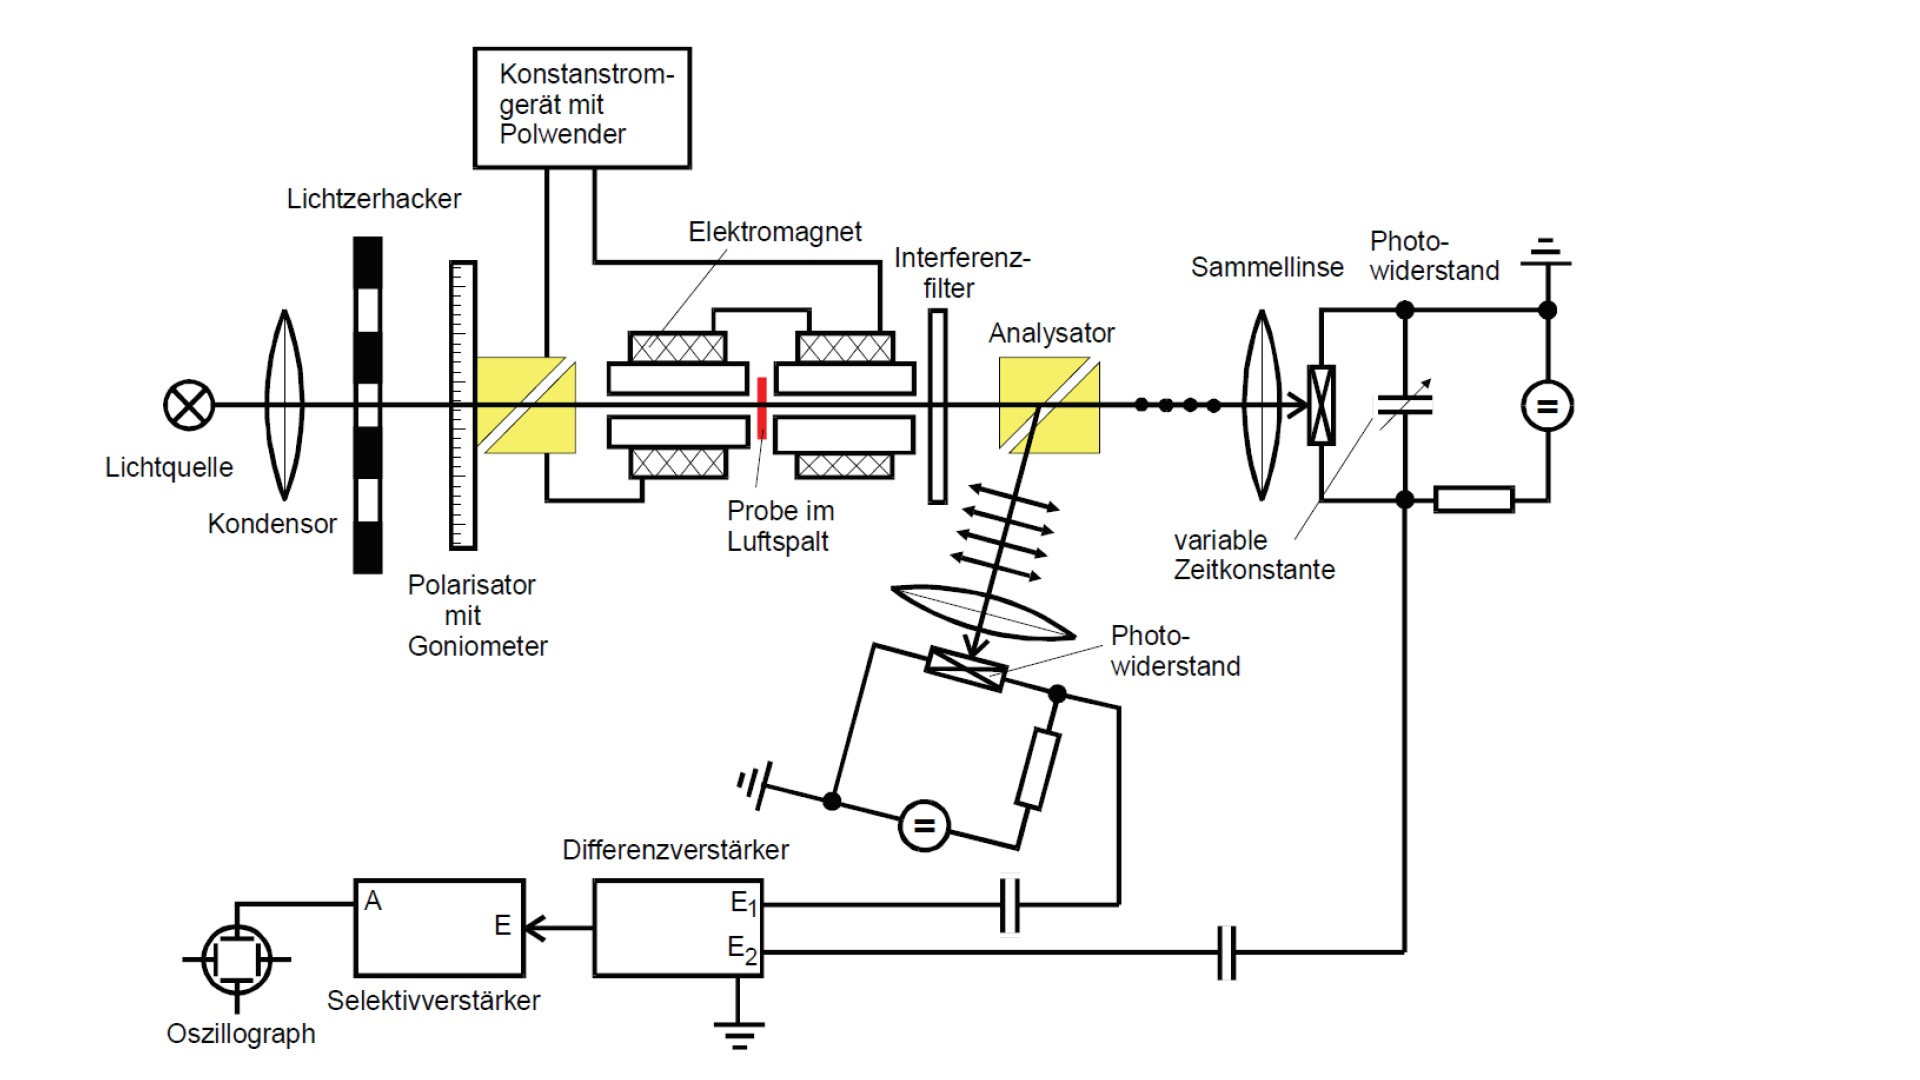
\includegraphics[width=1\textwidth]{bilder/aufbau.png}
  \caption{Schematische Darstellung des genutzten Versuchsaufbaus \cite{anleitung}.}
  \label{Aufbau}
\end{figure}
\subsection{Versuchsdurchführung}
\subsubsection{Justierung}
Zu Beginn des Versuchs muss der Aufbau justiert werden. Hierzu werden Probe, Interferenzfilter und die Abdeckungen der Photowiderstandgehäuse entfernt. Der Strahlenganz des Lichts wird überprüft und es wird getestet ob die Veränderungen am Goniometer die erwarteten Intensitätschwankungen an den Teilstrahlen verursachen.\\
Anschließend kann der Lichtzerhacker eingeschaltet und auf eine Frequenz von $450\si{\Hz}$ gestellt werden. Die Mittenfrequenz des Selektivverstärkers wird auf auf den Zerhacker angepasst indem man das Signal eines Photowiderstands am Differenzverstärker gegen ein "Ground"-Signal schaltet und das resultierende Signal in den Selektivverstärker gibt. Die Frequenz des Selektivverstärkers wird solange variiert bis man ein maximales Signal bekommt.
\subsubsection{Messung}
Zur Bestimmung des Drehwinkels wird eine Probe und ein Interferenzfilter in den Aufbau eingesetzt und es wird der Elektromagnet auf die maximale Leistung eingestellt. Mittels des Goniometers wird die Intensität der Teilstrahlen so eingestellt, dass das Signal am Oszilloskop Null wird. Ist dies erreicht so wird der am Goniometer eingestellte Winkel aufgezeichnet und das B-Feld wird umgepolt. Nun werden erneut die beiden Teilstrahlen abgeglichen und der eingestellte Winkel aufgezeichnet. Die Messung wird für Drei Proben und Neun Interferenzfilter durchgeführt. Abschließen wird noch die Stärke des B-Feldes mit einer Halls-Sonde bestimmt. 

\section{Auswertung}
Zur Bestimmung der Parameter der Probe ist es zunächst notwendig den Geometriefaktor $G$:
\begin{equation}
  G =
     \begin{cases}
       \frac{D}{\sin\left(\upalpha_i\right)}{d_0} &\quad\upalpha_i<\upalpha_g\\
       1 &\quad\upalpha_i\geq\upalpha_g
     \end{cases}
\end{equation}
zu berechnen. Hierbei ist $\upalpha_i$ der Einfallswinkel der Strahlung auf die Probe und $\upalpha_g$ der Geometriewinkel
\begin{equation}
\upalpha_g=\arcsin(\frac{d_0}{D}).
\end{equation}
$D=2\,\si{\cm}$ ist der Probendurchmesser und $d_0=0{,}2\,\si{\mm}$ die Höhe des Strahls. Der Geometriewinkel wird während des Justierens bestimmt und ist in diesem Fall $\upalpha_g=0.5717°$.
Durch Teilen der Messwerte durch den Geometriefaktor wird berücksichtigt, dass erst ab ausreichend großen Winkeln der gesamte Strahl die Probe trifft. Messwerte für sehr flache Winkel werden ausgelassen, da hierbei die Strahlung noch direkt in den Detektor treffen kann.\\
Zur Aufbereitung der Daten werden außerdem die Messdaten der Diffusionsmessung von denen der direkten Reflektionsmessung abgezogen. Zum Darstellen der aufgenommenen Messwerte werden die aufgenommenen Daten gegen den Wellenvektorübertrag $q_z=\frac{4\pii}{\lambda}\sin(\upalpha_i)$ aufgetragen. Hierbei ist $\lambda$ die Strahlungswellenlänge von $1{,}54\cdot10^{-10}\,\si{\m}$. Die Ergebnisse sind in Abb.\ref{Plot1} zu sehen.
\begin{figure}[H]
  \centering
  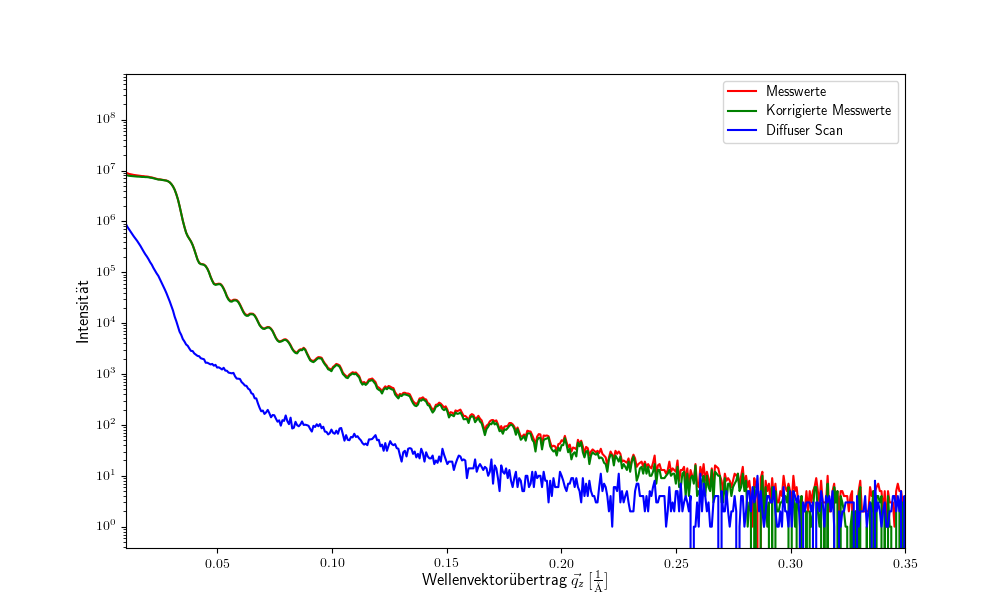
\includegraphics[width=\textwidth]{Berechnung/Plot1.png}
  \caption{Reflektivitätsscan aufgetragen gegen den Wellenvektor.}
  \label{Plot1}
\end{figure}
\subsection{Bestimmung der Probenparameter}
Zur Bestimmung der Probenparameter wird der Parratt-Algorithmus genutzt, um eine Theoriekurve an die  korrigierten Messwerte anzupassen. Die Schichtdicke $d$ lässt sich gemäß:
\begin{equation}
d=\frac{2\pi}{\upDelta q_z}
\end{equation}
bestimmen, indem die Periodendauer zwischen zwei Maxima vermessen wird. Durch die Lage des kritischen Winkels der Totalreflexion lässt sich danach der Brechungsindex des Substrates bestimmen. Die restlichen Parameter werden solange variiert, bis eine optimale Anpassung an die Messwerte erreicht wird. Hier ergibt sich für die Parameter damit:
\begin{align}
  \text{Brechungsindex Luft}:&\quad n_\text{Luft}=1\\
  \text{Brechungsindex Schicht}:&\quad n_\text{Schicht}= \left(1-1,2\right)\cdot10^{-6}\\
  \text{Brechungsindex Substrat}:&\quad n_\text{Substrat}=\left(1-7,4\right)\cdot10^{-6}\\
  \text{Rauigkeit Schicht}:&\quad \upsigma_\text{Schicht}=\left(15,5\right)\cdot10^{-10}\\
  \text{Rauigkeit Substrat}:&\quad \upsigma_\text{Substrat}=\left(9,8\right)\cdot10^{-10}\\
  \text{Schichtdicke}:&\quad z=873\,\AA
\end{align}
Die Kurve der korrigierten und normierten Messwerte sowie die des Parratt-Algorithmus sind in Abb.\ref{fit} dargestellt.
\begin{figure}[H]
  \centering
  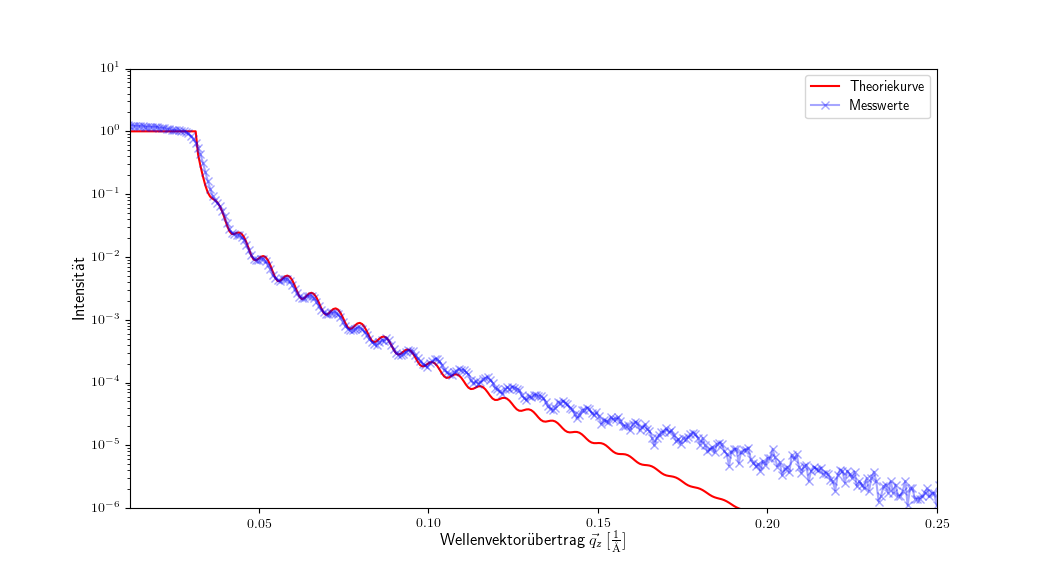
\includegraphics[width=\textwidth]{Berechnung/Fit.png}
  \caption{Kurve des Parratt-Algorithmus angepasst an die Messwerte.}
  \label{fit}
\end{figure}

\section{Diskussion}


\printbibliography

\end{document}
